\documentclass{article}
\usepackage{amsmath}
\usepackage{amssymb}
\usepackage{graphicx}
\usepackage{hyperref}
\usepackage[version=4]{mhchem}

\title{Problem 5}
\date{}

\begin{document}
\maketitle

\section*{Problem}
(AMC) Point \(E\) is selected on side \(A B\) of triangle \(A B C\) in such a way that \(A E: E B=1: 3\) and point \(D\) is selected on side \(B C\) so that \(C D: D B=1: 2\).


The point of intersection of \(A D\) and \(C E\) is \(F\). Then\\
\(\frac{E F}{F C}+\frac{A F}{F D}\) is (A) \(\frac{4}{5}\)\\
(B) \(\frac{5}{4}\)\\
(C) \(\frac{3}{2}\)\\
(D) 2\\
(E) \(\frac{5}{2}\)\\
\centering
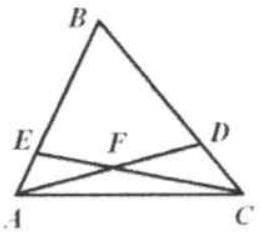
\includegraphics[width=\textwidth]{images/problem_image_1.jpg}

\section*{Solution}
(C).\\
Draw \(D H / / A B . \therefore D G: 3 a=b: 3 b ; D G=a=E A . \therefore E F=F G\) and \(A F=G D\), so that \(A F / F D=1\). Also \(D H: 4 a=b: 3 b, D H=\) \(4 a / 3\) and \(G H=D H-D G=a / 3 ; \therefore G C=\frac{1}{3} E C\) and \(E G=\frac{2}{3} E C\) and , since \(E F=F G, F C=\frac{2}{3} E C . \therefore\)\\
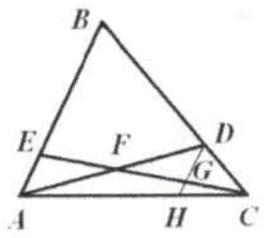
\includegraphics[width=\textwidth]{images/reasoning_image_1.jpg} \(E F / F C=\frac{1}{2}\).\\
\(\therefore \quad(E F / F C)+(A F / F D)=\frac{1}{2}+1=\frac{3}{2}\).\\

\end{document}
